\chapter{Similarity Distance Algorithms}
\label{ch:3}

In this chapter, we present seven different similarity distance measures. 
First, we describe four that are parameter-free, then we describe three algorithms that require a parameter. 
By chance, all of the parametric methods are based on Edit Distance, so we briefly explain how its construction as well. 


The methods have largely been chosen due to their prominence in the existing literature\cite{58-UCRTime,70-SimilarityDistances,8-EffectivenessStudy,53-TimeSeries,52-OnlineEfficient}. 
However, we present two newer algorithms, one parameter-free and one that requires a parameter.
They are presented at the end of their respective groupings. 
 
As was the case in the previous chapter, large portions here are based on the report created for \textit{TDT4501 Computer Science, Specialization Project}


\section{Parameter-Free Measures}
% The advantage of these parameter free methods is, as their names tell us, that they do not have parameters and they are “out of the box” ready. 

\subsection{Euclidean Distance (Ed)}
As noted in \Cref{ch:2}, the Euclidean distance (Ed) is a way to quantify the distance between two points in space. 
There is a naive extension of that principle that lays the foundation for a Euclidean Distance measure for trajectories\cite{44-FastSubsequence, 8-EffectivenessStudy, 24-ReviewTrajectory,86-ComputingMinimum}. This method would be to compute the mean point-point distances in a lock-step manner as seen in \Cref{eq:ed}.

\begin{equation}\label{eq:ed}
Ed(A, B) = \frac{1}{n}\cdot \sum_{i=1}^{n}d(a_i, b_i)
\end{equation}
where the distance between corresponding points is the $L_2$-norm as defined in \Cref{eq:l2norm}

Its simplicity comes with a couple of disadvantages, one notable one is that it requires the trajectories to be of equal length. 
In the cases where the number of points does not match one would have to adapt the data, potentially altering the original observations. 
Furthermore, computing distance in a lock-step manner means that it is sensitive to local time shifts and noise\cite{12-RobustFast}. 

Even with these limitations, this measure is included for its simplicity.  Previous work has shown that it holds remarkably well up to more advanced methods\cite{26-QueryingMining}, further encouraging us to examine this metric. 


\subsection{Dynamic Time Warping (DTW)}

As stated in \Cref{sec:elasticity} an elastic measure is needed in order to handle local time shifts and Dynamic Time Warping (DTW) is precisely that. 
DTW was originally designed for speech recognition which means that it handles relative lag seamlessly\cite{45-CrosswordsReference, 27-DynamicTime}.
This makes it a prevalent choice for examining similarity under temporal drift.
The idea behind this algorithm is to stretch and contract time such that a favorable alignment of the input trajectories can be found. 


\Cref{fig:dtw_cost_path} illustrates the implementation of DTW. 
The computation begins by taking input trajectories $A$ and $B$ and constructing a full cost matrix $C$. This matrix keeps all pairwise distances  between the trajectories' elements. 
We use the $L_2$ norm for point-to-point distance computation as is common for DTW\cite{5-ComputingVisualizing}. 
After the matrix has been constructed, the next step is to iteratively search through  $C$ and find the optimal warping path, $p$. 
The optimal warping path is the set of point-point pairings, entries of $C$, that  minimizes the accumulated cost. 
The accumulated cost along the warping path is the DTW distance between the trajectories. 
\Cref{fig:ed_dtw_diff} exemplifies how the Euclidean distance and DTW differ with respect to time-shift. 

% how this approach stands out from 
% for an illustration of how the points are aliened under a lock-step measure like the Euclidean Distance and DTW.

\begin{figure}[h]
\centering
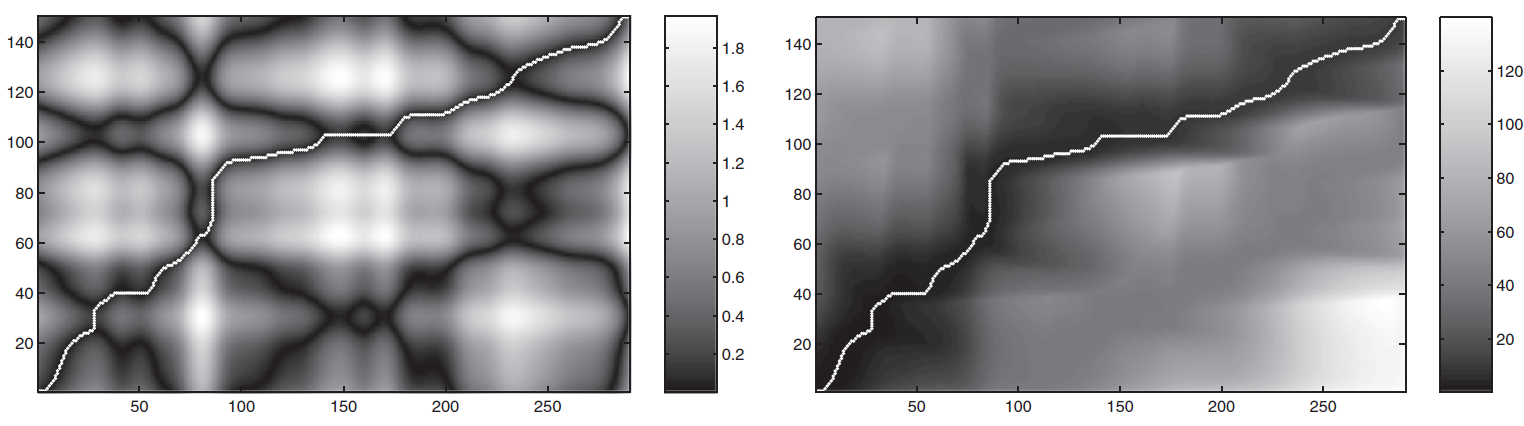
\includegraphics[width=.7\textwidth]{figs/algos/dtw_C_p.png}
\caption{Cost matrix $C$ (left) and accumulated cost matrix $C'$ which the optimal warping path $p$ (right) . Figure copied from \cite{27-DynamicTime}}
\label{fig:dtw_cost_path}
\end{figure}

\begin{figure}
\centering
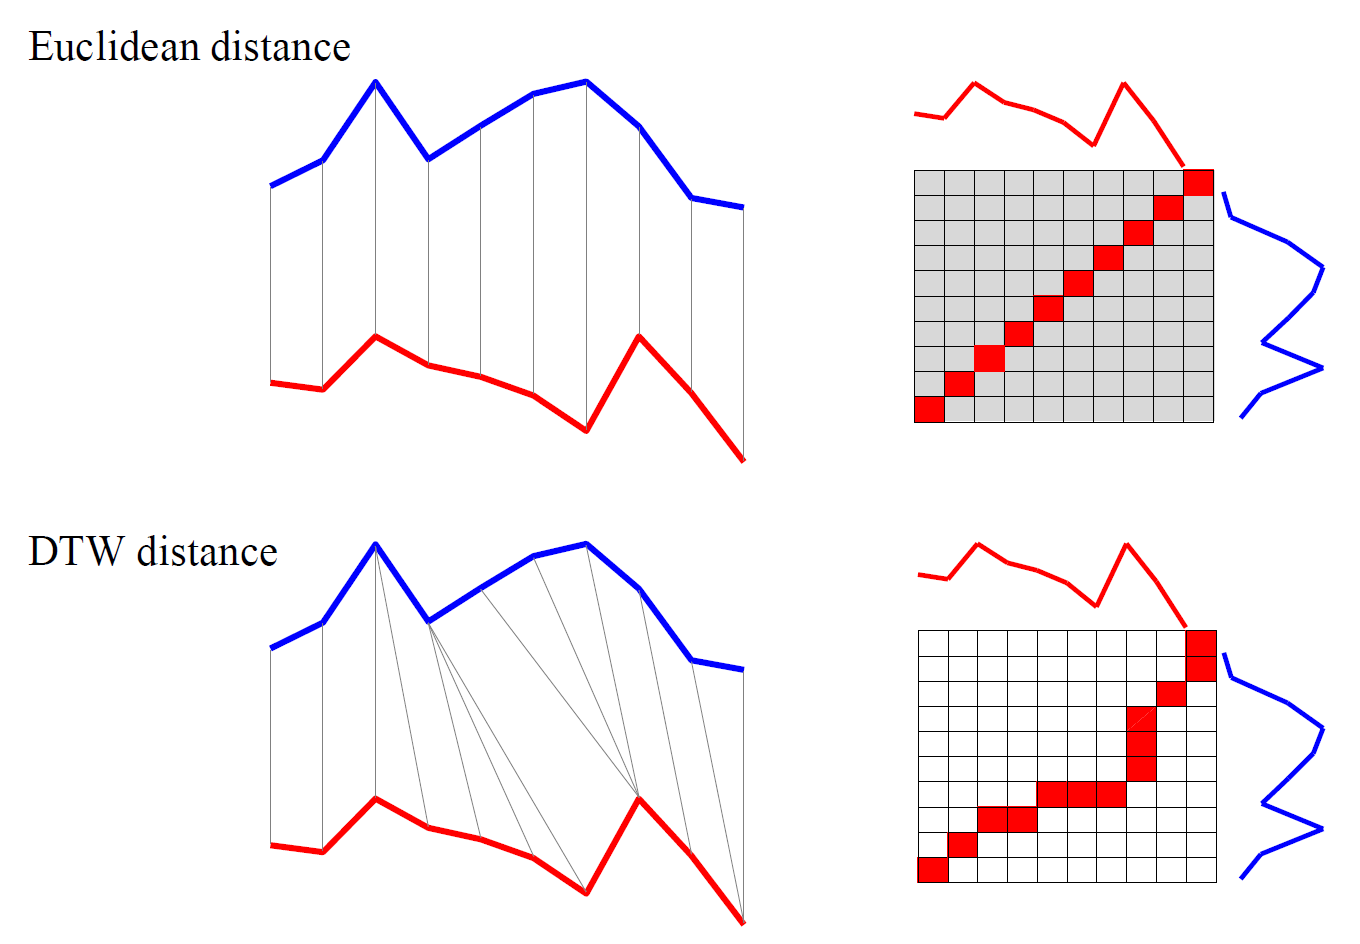
\includegraphics[width=.7\textwidth]{figs/algos/ed_dtw_diff.png}
\caption{An illustration of how the Euclidean forces a lock-step computation whereas DTW realigns the trajectories. Figure copied from \cite{58-UCRTime}}
\label{fig:ed_dtw_diff}
\end{figure}


The main drawback of DTW is that it weights all points of both trajectories equally and thus it is not robust to noise. 
A naive implementation of DTW would forcefully align the start- and endpoints of the two trajectories which can disproportionately punish trajectories that are overall similar\cite{4-ElasticPartial}. 
Generating the cost matrix quickly becomes expensive due to pairwise comparing all points of the input trajectories which makes it less suited for large data sets \cite{27-DynamicTime}. 

Its shortcomings have inspired iterations of DTW that seek to address them. Some remark that constructing a full cost matrix may not be needed, and some seek to speed up how to iterate through $C$\cite{5-ComputingVisualizing}. We note that a popular choice is \textbf{FastDTW}, which is a parameterized version of DTW. 
As the name indicates, it is much faster than the naive implementation yet gives comparably accurate results\cite{9-FastDTWAccurate}. 
Nevertheless, this thesis shall only focus on the parameter-free version.



\subsection{Hausdorff Distance (Hd)}
% This distance measure is a metric that weights shape similarity, meaning the temporal aspect or order of trajectory elements does not matter 
This technique is often discussed in relation to polygons and sets\cite{49-HausdorffDistance} however it is applicable for time-series data as well. 
A consequence of its geometric origin is that the trajectory direction no longer affects the final result, the notion of a first or last trajectory element is not kept\cite{86-ComputingMinimum}. 
The Hausdorff distance from  $A$ to $B$ is the maximum of the minimum of all pairwise distances, see \Cref{eq:Hd-directed}\cite{48-ComputationalGeometrya} 

\begin{equation}
\label{eq:Hd-directed}
\widetilde{Hd}(A, B) = max_{a\in A}\big\{ \, min_{b\in B } \enspace d(a, b)\,\big\}
\end{equation}

where $d(a, b)$ is any metric distance function, here the $L_2$-norm is used. 
The distance function described in \Cref{eq:Hd-directed} is not symmetric and thereby not a metric\cite{14-EfficientAlgorithm}. The function is referred to as the directed Hausdorff distance. 
To make the Hausdorff metric, it is defined as the maximum  of the two directed results. 
This makes the function symmetric, so that it fulfills the requirements for a metric, see \Cref{eq:Hd-metric}.

\begin{equation}
\label{eq:Hd-metric}
Hd(A, B) = max\big\{ \,\widetilde{Hd}(A, B), \;\widetilde{Hd}(B, A)\big\}
\end{equation}

Since we can compare any point in A to any point in B this measure is elastic. 
All points of the trajectories are weighted equally which makes it is sensitive to noisy data. 
Additionally, the effect of reducing the similarity score to the distance between two points from each trajectory is that information about the trajectories' overall shape is lost. 
The metric is highly sensitive to noise\cite{51-HausdorffDistance}. 
Lastly, we need to work out both of the directed distances to get the similarly score. This means more work per trajectory pair than naturally symmetric measures such as Ed and DTW.  


\subsection{Symmetrized Segment-Path Distance (SSPD)}
As the  Hausdorff distance, Symmetrized Segment-Path Distance (SSPD) method is a spatial only algorithm that largely disregards the direction of the trajectories.
It is was developed from the same principles as the Hausdorff distance, but with the addition of being able to account for  the trajectories as a whole.\cite{43-TrajectoryDistance, 50-ReviewPerspective}. 
The algorithms explained so far have used the trajectory elements directly as the basis for the computations. For SSPD, this is no longer the case, and thus we define notation and terms to describe this algorithm.  

 In line with  \Cref{tb:notation}  $a, b$ are elements of Trajectories $A, B$ respectively . 
 A \textit{segment} is the line between two consecutive points, and we use $\breve{a}$ to denote a segment of $A$. Using indexes,  $\breve{a}_i$ is the line between $a_i$ and $a_{i+1}$. 

Next we define the \textit{point-to-segment distance} as shown in \Cref{eq:sspd-ps}. This distance function requires us to find the point’s orthogonal projection onto the segment. 
If it is within the segment, the distance will be the  $L_2$-norm between the original point $a$ and its projection $\dot{a}$.
Otherwise, the  $L_2$- norm to segment's end points is computed nearest those distances becomes the point-to-segment distance.  

\begin{equation}
\label{eq:sspd-ps}
d_{ps}(a_i, \breve{b}_j) =  \begin{cases}
d(a, \dot{a})  &\text{if} \enspace \dot{a} \in \breve{b}_j\\
min\{ d(a_i, b_j), d(a_i, b_{j+1})\}  &\text{otherwise}
\end{cases}
\end{equation}
Where $\dot{a}$ is the orthogonal projection of point  $a$ onto segment  $\breve{b_j} $ and $d$ is the $L_2$-norm. 

From point-to-segment distance, \textit{point-to-trajectory distance} is defined as shown in \Cref{eq:sspd-pt}. 
The point-to-segment distance is computed for all the segments of the trajectory and the lowest one becomes the point-to-trajectory distance.

\begin{equation}
\label{eq:sspd-pt}
D_{pT}(a_i, B) = min_{\breve{b} \in B} \big\{ \, d_{ps}(a_i, \breve{b})\, \big\}
\end{equation}
The \textit{Segment-Path-Distance} (SPD) is directed.
It is defined to be the mean of the all point-to-trajectory distances from points of the first trajectory to the second trajectory, \Cref{eq:sspd-spd}.

\begin{equation}
\label{eq:sspd-spd}
SPD(A, B) = \frac{1}{n_A} \sum_{i=1}^{n_A} D_{pT} (a_i, B)
\end{equation}
As with the Hd, this distance measure is made symmetric by computing both directed versions first. However unlike Hd, the final result is the mean of the directed results. The name comes from this last step and the final formula is shown in \Cref{eq:sspd-main}.
 
 \begin{equation}
\label{eq:sspd-main}
SSPD(A, B) = \frac{\big( \, SPD(A, B) + SPD(B, A)\, \big)}{2}
\end{equation}

 
The creators of SSPD note that if one were to use the max function rather than computing the mean upon symmetrification this algorithm would be identical to the Hausdorff function\cite{50-ReviewPerspective}. 
They note that with their method, this distance function becomes more robust to noise when calculating the mean, as opposed to maximizing or minimizing.  
Moreover, they commend SSPD for being parameter-free as well as not relying on interpolation between two observed point, preferring to strengthen the importance of observed data. 
As a closing remark, we note that SSPD does not fulfill the requirements of a metric. 

\section{Parameterized Measures}


 In this section, we have described measures that require a parameter. 
 All of them are based on String Edit Distance (SED) which is a similarity measure designed for strings.  
 The idea is to count the number of \textit{edits} needed to convert one string into the other using the edit operations are insert, delete and replace.  
 Due to the strings' natural discretization, it is trivial to determine whether or not two symbols are matching. 
There are variations of implementation but a common choice is to let the cost of an \textit{edit} be 1, creating a formula as seen in \Cref{eq:ed_string}:  

\begin{equation}\label{eq:ed_string}
    \text{SED}(S1, S2) = \begin{dcases}
        \quad |S1| & \text{if }  |S2| = 0\\
     	\quad |S2| & \text{if }  |S1| = 0\\
        \quad \text{SED}(S1,\; S2) & \text{if }  |S1| =|S2| \\
        \begin{aligned}
        1 + min\big\{   & \text{SED}(Rest(S1), \; Rest(S2)) \\
              	     & \text{SED}(Rest(S1), \; S2) \\
           		    & \text{SED}(S1, \; Rest(S2)) \\
        \end{aligned} & \text{otherwise}
  \end{dcases}
\end{equation}

Real data does not let itself be discretized as fortuitously as strings, thereby leading to the creation of the algorithms below. 
The measures differ in how they have adapted SED for time series data, and the role of the parameter value changes as well. 
 

% \subsection*{FastDTW}
% As its name indicates, this algorithm is a modification of DTW. We remarked that DTW is expensive in both time and space complexity. FastDTW archives linear complexity on both fronts, but does introduce a parameter to do so \cite{9}. 

% The idea behind this is to first run the algorithm at coarse resolution, compute a projected warp-path and then rerun the algorithm at a finer resolution to tune the path. This is repeated until we have reached the original resolution. Two of the most important ways this algorithm is sped up are the following. 
% Firstly, fewer cells of the cost matrix need to be calculated or evaluated. Secondly, data abstraction means that the cost of DTW itself is greatly reduced. This means a great improvement in cost, however at the expense of no longer being parameter free. The parameter in question is a radius parameter which determines how much the projected optimal path can deviate from the one found at the previous iteration. See FIGURE for an illustration of how the iterative search plays out with the radius parameter. WILL NOT INCLUDE


% One way we could speed up DTW is by introducing a \textit{radius parameter}, and this algorithm is called FastDTW\cite{9}. This approach first runs the algorithm at a coarser resolution, and then reruns itself in order to tune the result. This means a great improvement in cost, however at the expense of no longer being parameter free. Nevertheless we have chosen to include both DTW and FastDTW as part of our survey to examine the impact of this alteration. 

\subsection{Edit Distance on Real Sequence (EDR)}

Edit Distance on Real Sequence (EDR)\cite{12-RobustFast} introduces a threshold parameter $\epsilon$ that determines if two trajectory elements are “matching”. 
Crucially, there can be no partial matches so the point-to-point distance is either 1 or a 0 as shown in \Cref{eq:edr_subcost}.

\begin{equation}\label{eq:edr_subcost}
d_{edr} (a, b) = \begin{cases}
0 \quad &\text{if } \quad | a_{LNG} -b_{LNG}|\leqslant  \epsilon  \text{ and } | a_{LAT} -b_{LAT}|\leqslant  \epsilon    \\
1 \quad &\text{otherwise}\\
\end{cases}
\end{equation}
where $\epsilon$ is the threshold parameter. After determining whether or not two points match with the subcost function we get the full EDR is shown  algorithm as seen in \Cref{eq:edr_main}


\begin{equation}\label{eq:edr_main}
    EDR(A, B) = \begin{cases}
        n_A \qquad &\text{if } n_B = 0\\
        n_B \qquad &\text{if } n_A = 0\\
        \begin{aligned}
        min\big\{ & EDR(\text{ Rest}(A), \text{ Rest}(B)) + d_{edr}(a, b),\\
              & EDR(\text{ Rest}(A), B) + 1,\\
              & EDR(A, \text{ Rest}(B)) + 1 \big\}
        \end{aligned} & \text{otherwise}
  \end{cases}
\end{equation}where $a, b$ are the leading elements of $A, B$.  

The main advantages of EDR are its resistance to noise and the ability to handle local time shifts. 
It is resistant to noise because of how it maps the distance between elements to a binary 1 or 0. 
Toohey and Duckham asserted that EDR performed well in spite of variance in the sampling rate\cite{17-TrajectorySimilarity}.

EDR is not a metric measure as it does not fulfill triangle inequality, but it meets other requirements of metrics. 
Furthermore, it evaluates similarity as trajectory elements, not taking into account the trajectories' overall shape. 
We have chosen to include this algorithm as it is a well-studied algorithm. 
Its prevalence in the literature has led it to be studied alongside DTW and Euclidean Distance. 


\subsection{Edit Distance with Real Penalty (ERP) }
Edit Distance with Real Penalty (ERP) was designed to bridge the gap between metrics distance functions and local time shifting tolerant ones. \cite{13-MarriageLpnorms}. The design of EDR began with the $L_1$-norm \Cref{eq:manhatten}

\begin{equation}\label{eq:manhatten}
Dist_{L1} (A, B) = \sum_{i=1}^{n} d(a_i, b_i) \qquad \text{where} \qquad d_{L_1}(a_i, b_i) = \sum_{j=1}^{p}|a_{i,j}- b_{i,j}|
\end{equation}

From SED, the notion of a \textit{gap element} is introduced. 
A gap element is a symbol that could have been deleted from string $S1$ but instead is inserted into string $S2$.
The point-to-point distance function would then become what is shown in \Cref{eq:erp_ed}. 

\begin{equation}\label{eq:erp_ed}
    d_{ed}(a_i, b_i) = \begin{cases}
        0 &\qquad \text{if } a_i = b_i \\
        1 &\qquad \text{if } a_i \text{ or } b_i \text{ is a gap } \\
        1 &\qquad \text{otherwise } \\
    \end{cases}
\end{equation}

% SED, just as the $L_p$ norms, is a metric distance measure, but to further develop this algorithm it needs to accommodate real values.
Rather than using a constant value to penalize all edit operations uniformly like EDR, ERP differentiates between gap elements and non-gap elements. 
This distinction is important so that it will be tolerant to local time sifting. 
Gap elements are penalized with a constant value, while non-gap elements have a real-value cost based on their value. 
The parameter of ERP,  $g$, is the reference value for cost computation, and the point-to-point distance function is seen in \Cref{eq:erp_sub}

\begin{equation}\label{eq:erp_sub}
     d_{epr}(a_i, b_i) = \begin{cases}
        |a_i-b_i| & \qquad \text{if  neither is a gap} \\
        |a_i-g|   & \qquad \text{if } b_i \text{ is a gap} \\
        |b_i-g|   & \qquad \text{if } a_i \text{ is a gap} \\
     \end{cases}
 \end{equation}
 
 Again, the trajectory distance function is an adaption of SED, and the full algorithm for ERP is shown in \Cref{eq:erp_main}
%  but was no longer a metric after it.
\begin{equation}\label{eq:erp_main}
    ERP(A, B) = \begin{dcases}
        \quad \sum_{i=1}^{n_A}|a_i - g| & \text{if }  n_B = 0\\
        \quad \sum_{i=1}^{n_B}|b_i - g| & \text{if }  n_A = 0\\
        \begin{aligned}
        min\big\{   & {ERP}(Rest(A), \; Rest(B)) + d_{erp}(a_1,\;  b_1),\\
              	    & {ERP}(Rest(A), \; B) + d_{erp}(a_1, \; g),\\
           		    & {ERP}(A, \; Rest(B)) + d_{erp}( b_1,\; g) \big\}
        \end{aligned} & \text{otherwise}
  \end{dcases}
\end{equation}

The main drawback of this method stems from the characteristic that makes it a metric, using differences of real values as costs.
This method is a metric as long as $g$ is constant, making the cost of an edit vary the location of the trajectory element. 
However, this makes ERP sensitive to noise\cite{12-RobustFast}. 


\clearpage
\subsection{Move-Split-Merge (MSM)}
Move-Split-Merge (MSM) \cite{40-MoveSplitMergeMetric} is similar to the aforementioned to the other SED-based approaches in that it calculated the similarity score from how many operations are needed to transform one trajectory into another one.
This algorithm is tolerant to temporal misalignments and translation invariant\cite{53-TimeSeries} as are EDR and ERP.  
What distinguishes this algorithm from them is how insertions and deletions are handled.
The MSM cost model uses both the value of the element being modified as well the adjacent one whereas ERP only uses the element being modified and EDR uses a constant cost for all operations. 


As the name of this algorithm indicates, the possible operations are Move, Split, and Merge, which are then used to emulate the established Edit Distance operations Insert, Delete, and Substitute.
The Move operation is a renaming of does the same as Substitute.
The Split operation inserts a copy of a given value directly after itself, and the Merge operation deletes a value if it is immediately followed by a matching value\cite{53-TimeSeries}. In other words, Split and Merge are each others’ inverse.
The Insert operation becomes a Split followed by a Move, while Delete becomes a Move followed by a Merge. 
The MSM parameter, $c$, is  a non-negative value that determines the cost of every Split and Merge operation. See \Crefrange{eq:msm-start}{eq:msm-end} for details. 

\begin{align}
 A  &= [a_1, \cdots , a_{i-1},\, a_i,\, a_{i+1}, \cdots  , a_{n_A}] \nonumber \\
 \nonumber\\
\text{Move}_{a_i \rightarrow b_j}(A)  &= [a_1, \cdots , a_{i-1},\, b_j,\, a_{i+1}, \cdots  , a_{n_A}] \label{eq:msm-start} \\
\text{Cost} \big\{ \text{Move}_{a_i \rightarrow b_j}(A) \big\} &= d(a_i, b_j) \\
\nonumber \\
\text{Split}_{a_i}(A) &= [a_1, \cdots , a_{i-1},\,a_i,\, a_i,\, a_{i+1}, \cdots  , a_{n_A}]\\
\text{Cost} \big\{ \text{Split}_{a_i}(A) \big\} &= c \\
\nonumber \\
\text{Merge}_{a_i}(A) &= [a_1, \cdots , a_{i-1},\, a_{i+1}, \cdots , a_{n_A}] \\
\text{Cost} \big\{ \text{Merge}_{a_i}(A) \big\} &= c \label{eq:msm-end}
\end{align}

Recall that the $\text{Merge}_{a_i}(A)$ operation is only permitted if $a_i = a_{i+1} $. 
This algorithm fulfills the requirements of a metric and thus it can be used for indexing and clustering techniques that are designed to function in metric spaces. 
In terms of computational cost and accuracy, we refer to work done by Bagnall et. al. which alludes to MSM being comparably efficient to ERP and more tolerant to noise DTW\cite{56-GreatTime}.

 

 
 \clearpage
\section{Summary of Algorithms}

\Cref{tab:meas_comp} summarizes some trajectory similarity features. 
Remark that none of the measures have matching rows, further indicating that the meaning of trajectory similarly varies with technique implementation. 


We reiterate that large portions of this chapter stem from the report that was mentioned at the beginning. 
Still, there is not a complete overlap of the measures discussed in that report and this thesis. 



% Euclidean distance is the only measure that does not account for local time shifts, and    
% From all aspects apart from "overall shape" similarity, there has been about half and half if they measures fulfilled the requirements.

% distance functions satisfy the requirements of metricity 

% https://www.tablesgenerator.com/latex_tables

\begin{table}[t]
\centering
\caption{Quick view of some aspects the similarity distance measures}
\label{tab:meas_comp}
\resizebox{\textwidth}{!}{%
\renewcommand{\arraystretch}{1.5}
\begin{tabular}[h]{*{6}{|p{1.8cm}}|}
 \hline
\textbf{Name}   & \textbf{Metric } & \textbf{Single \newline Element } & \textbf{Time Shifts} & \textbf{Parameter} & \textbf{Noise \newline Tolerant}      \\ 
\hline
\textbf{ED} 		 & Yes    & Yes     & No  & No    & No      \\ 
\hline
\textbf{DTW}      & No:    &Yes    &Yes    & No   & No    \\ 
\hline
\textbf{Hd}       & Yes    & Yes        &Yes     & No     & No      \\
\hline
\textbf{SSPD}      & No    & No          &Yes   & No   & Yes  \\ 
\hline
\textbf{EDR}       & No   & Yes    & Yes       & Yes     & Yes   \\
\hline
\textbf{ERP}       & Yes   & Yes    & Yes      & Yes    & No    \\
\hline
\textbf{MSM}      & Yes   & No    & Yes   & Yes   & Yes \\ 
\hline
\end{tabular}
}
\end{table}


% double check the noise tolerances, use checkmarks?
